\section{Android architecture}

Android is an open source operating system, based on the Linux kernel and created to fit multiple types of devices \cite{noauthor_platform_2023}.
Android applications (or \textit{apps}) are written using programming languages that compile for the Java Virtual Machine (JVM) bytecode, such as Java or Kotlin. The JVM bytecode is compiled to a Dalvik Executable (DEX) bytecode format, and is then packaged along with other application resources to form an Android Application Pack (APK) file, which can be distributed for end-users. The app building process can be seen at Figure \ref{fig:android-build}.

\begin{figure}
    \centering
    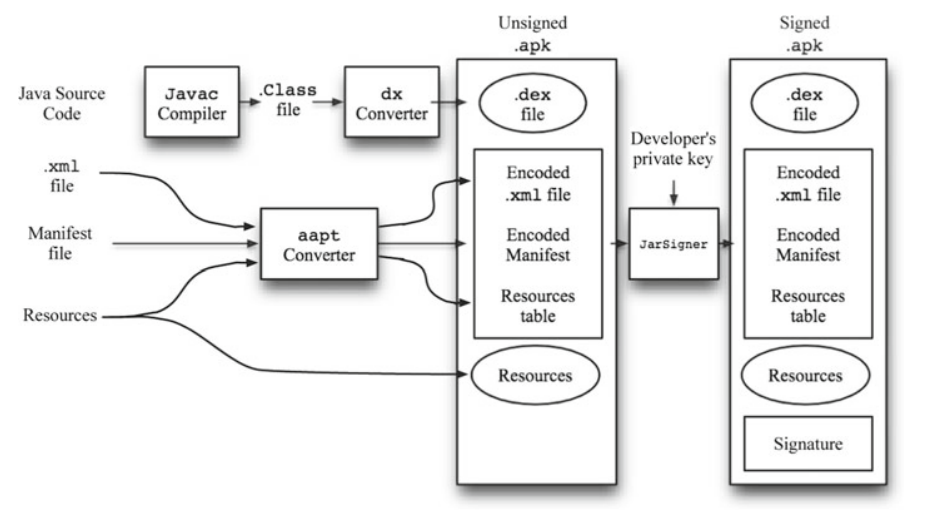
\includegraphics[width=\textwidth]{img/android_build.png}
    \caption{Android build process, from source code to APK file. Source: \cite{jung_repackaging_2013}.}
    \label{fig:android-build}
\end{figure}

The Android platform identifies and isolate each individual app and its resources, by assigning them a unique identifier (UID) and running each Android app on its own process~\cite{noauthor_application_2022} of the Android Runtime virtual machine, which interprets the DEX bytecode. The assigned UID is used to establish a kernel-level application sandbox, that isolates every app from each other, protecting both the apps and the system from malicious activity.

In order to access information beyond the application sandbox, apps must acquire permissions and then access the resources through specific system Application Programming Interfaces (APIs). Android has two main types of permissions \cite{noauthor_permissions_2023}: install-time permissions, and runtime permissions. Install-time permissions are less sensitive permissions and must be requested upon installation of the APK on the system, such as internet access. Runtime permissions are highly sensitive permissions and are generally related to users' private data, such as camera or microphone access. Runtime permissions must be acquired right before the actual use of the resource, and are only available on Android 6.0 or higher.


\section{Android malwares}

A \textit{malware} is a type of application that's capable of executing code that may carry out harmful activities on a system, its modules, or other applications. It's defined as a ``set of instructions that run on your computer and make your system do something that an attacker wants it to do'' \cite{skoudis_malware_2003}. Mobile devices have evolved to perform activities that were only possible on desktop computers, such as internet access or banking, along with having its own set of features such as calling, SMS, access to precise location, or high quality cameras and microphones and for that reason they are a huge target for malware and other types of malicious attacks.

Zhou et al. \cite{zhou_dissecting_2012} characterizes Android malware based on their installation, activation and the carried malicious payloads. The techniques used by the malware to install onto the user devices were analyzed, and separated on three main groups: \textit{repackaging}, \textit{update attack} and \textit{drive-by download}, which aren't necessarily mutually exclusive. Regarding the activation mechanisms, the existing Android events were examined to determine how malware used them to flexibly trigger their activation (e.g., only starting its background services when the system is started). Finally, the payloads were also analyzed and classified in four major categories: \textit{privilege escalation}, \textit{remote control}, \textit{financial
charges}, and \textit{personal information stealing}.

Although the isolation provided by the application sandbox and restrictions enforced by the permission mechanism add a layer of protection for Android devices, they are not flawless. Felt et al. revealed that around 33\% of Android apps are overprivileged and the developers fail to achieve the least privilege principle \cite{felt_android_2011}. Moreover, a portion of the users do not pay enough attention to the required permissions of the apps they install~\cite{felt_android_2012}.

\section{Repackaging malwares}

Repackaging is one type of attack on the Android ecosystem, and \cite{zhou_dissecting_2012} have shown that the majority (around 86\% on the analyzed dataset) of Android malware make use of this type of attack. It consists on gathering an existing application, reverse engineering its code, inserting a malicious activity and then publishing the modified (i.e. repackaged) application on app marketplaces. Once a repackaged app is installed on an Android device and is granted the requested permissions, malicious actors can then collect private user data, perform malicious activities and exploit any other actions allowed by the granted permissions. 

Since the application code is compiled to a DEX bytecode, some characteristics about the original code such as class names, method names, and types are retained, which makes them more susceptible for reverse engineering if compared to native code \cite{hamilton_evaluation_2009}.

\section{The Mining Android Sandbox (MAS) technique}

% talk about Jamroski and his work with Boxmate
The mining sandboxes approach for the Android platform was first proposed by Jamroski et al. and consists of exploring the behaviour of software by extracting the accessed resources through an automated test generation, and then constructing a sandbox based on those resources \cite{jamrozik_mining_2016}. This ``mined'' sandbox would then prevent and detect unexpected behaviour changes, such as latent malware, infections, malicious updates, etc.

Jamroski et al. introduced a tool called \textit{Boxmate}, that performs such mining sandbox technique, and creates a resulting sandbox much more fine-grained than the original sandbox present on the Android operating system. Boxmate uses a tool called \textit{Droidmate} as test generation tool. However, this study only evaluated the effectiveness of this technique on benign apps, and didn't investigate if it was effective in detecting malware.

% talk about "mining sandboxes: are we there yet?"
This study was then complemented by Bao et al., that evaluated the effectiveness of the mining sandboxes technique on detecting malicious behaviours on Android apps, and investigated the effectiveness of test generation tools for mining sandboxes \cite{bao_mining_2018}. It makes use of a set of pairs of apps where each pair consist of a benign app and a malicious repackaged version of the same app. Bao et al.'s study shows that up to 75.5\% of the malicious versions of the apps can be identified using the mining sandboxes approach. It also shows that DroidBot \cite{li_droidbot_2017} is the most effective test case generation tool among the tested options, which included Monkey, Droidmate, Droidbot, GUIRipper, and PUMA.

%\section{Previous works}

%...

\section{DroidFax}

DroidFax is an open-source toolkit that instruments Android apps and performs a series of analyses (both static analysis and dynamic analysis through test case generation tools) on the application execution structure and sensitive data accesses at runtime. It was developed by Cai H. to perform a study on Android apps runtime characteristics and their security implications \cite{cai_understanding_2016}. 

Costa et al. \cite{costa_exploring_2022} investigated the impact of DroidFax's static analysis algorithms for malware identification, and how it can complement the malware detection capabilities of the MAS approach presented by Bao et al.'s study \cite{bao_mining_2018}. Costa et al.'s study have shown that 43\% of the malware could be detected using the static analysis alone.

DroidFax instrumentation runs on top of Soot \cite{vallee-rai_soot_1999, noauthor_soot_nodate}, a framework to analyze, instrument and optimize Java bytecode. The instrumentation is made by transforming the bytecode in an intermediate representation (Jimple, in the case of DroidFax), analyzing and manipulating (by adding logs, for example) the source code, and finally producing the modified bytecode.

\section{DroidXP}

%tell the reader about the droidxp, it's architecture and how it's used for sandbox mining approach
DroidXP is a benchmarking suite developed by Costa et al. at \cite{costa_droidxp_2020} and its initial goal was to provide a software infrastructure that's capable of comparing the performance of multiple test case generation tools on mining sandboxes for the Android platform. It relies on DroidFax as instrumentation and static analysis tool, and supports many test case generation tools out of the box for the dynamic analysis (and can be easily extended to support other tools). The benchmark is performed on three main phases, as illustrated by Figure \ref{fig:droidxp-arch}, which are performed after the user specifies the test case generation tool, the number of repetitions for every app version, and the test execution period:

\begin{enumerate}
    \item Phase one -- Instrumentation: in this phase, DroidXP makes use of DroidFax to perform the instrumentation and static analysis on the app pairs provided by the user.
    \item Phase two -- Execution: then, DroidXP installs the instrumented apps on an Android emulator and runs the test case generation tool for the specified period of time, for every specified repetition. During the execution, all the logs produced by the DroidFax dynamic analysis is collected using Android SDK's logcat \cite{noauthor_logcat_2023}. The emulator is fully reset after every app execution, to ensure that no executions interfere with each other.
    \item Phase three -- Report: finally, DroidXP analyzes the results of both static and dynamic analysis and generates the experiment results, which includes the code coverage of the test case generation tool and the sensitive Android APIs accessed by each version of each app.
\end{enumerate}

\begin{figure}
    \centering
    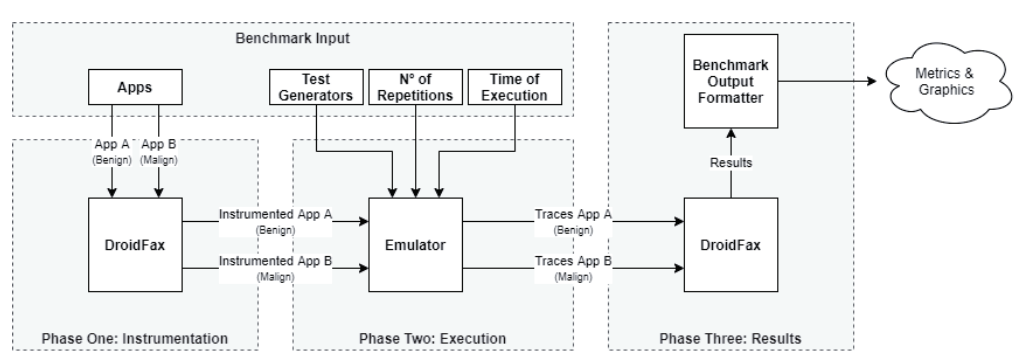
\includegraphics[width=\textwidth]{img/droidxp.png}
    \caption{DroidXP benchmark architecture. Source: \cite{costa_droidxp_2020}.}
    \label{fig:droidxp-arch}
\end{figure}

DroidXP further improved by Costa et al. \cite{costa_exploring_2022}, to investigate the impacts of using both static and dynamic analysis for Android malware identification.